\documentclass{sig-alternate}
%[preprint]
% The following \documentclass options may be useful:
%
% 10pt          To set in 10-point type instead of 9-point.
% 11pt          To set in 11-point type instead of 9-point.
% authoryear    To obtain author/year citation style instead of numeric.

\makeatletter
\def\@copyrightspace{\relax}
\makeatother

\usepackage[nynorsk,british,UKenglish,USenglish,english,american]{babel}

\usepackage{graphicx}
\usepackage{tikz}
%\usepackage{gnuplot-lua-tikz}
\usepackage{color}
\usepackage{tabularx}
\usepackage{fixltx2e}
%% \usepackage{dblfloatfix}
\usepackage{varwidth} % http://ctan.org/pkg/varwidth
\usepackage{listings}
\usepackage{url}
\usepackage{balance}
\usepackage{amsmath}
\usepackage{enumitem}
\usepackage{caption}

\lstset{
%  backgroundcolor=\color{yellow!20},%
  basicstyle=\small\ttfamily,%
  numbers=left, numberstyle=\tiny%
}

\newtheorem{thm}{Problem}
\newdef{definition}{Definition}
\DeclareMathAlphabet{\mathpzc}{OT1}{pzc}{m}{it}
\newtheorem{theorem}{Theorem}[section]
\newtheorem{lemma}[theorem]{Lemma}

\usepackage{xcolor}
\usepackage{framed}
\usepackage{amssymb,amsmath}
\usepackage{ifxetex,ifluatex}
\usepackage{fancyvrb}
\usepackage{comment}

\begin{document}

\title{\Large\bf Design an accelerator for Computing MRI-Q Matrix}
\subtitle{\normalsize COMS E6868 - Embedded Scalable Platforms - Spring 2020}

\numberofauthors{1}
\author{
\alignauthor
Pei Liu\\
\vspace{0.2cm}
       \email{pl2748@columbia.edu}
}

\vspace{-2cm}

\maketitle

\vspace{-2cm}

\begin{abstract}
{\small\em
  I plan to design an accelerator to calculate the Magnetic Resonance Imaging Q matrix through SystemC and HLS tool Stratus and implement this design on FPGA. Then I plan to explore the design space to get a thorough understanding of the methodology of designing accelerators though ESP. 
}
\end{abstract}

\section{Introduction}
\label{sec:intro}
Magnetic Resonance Imaging is commonly used by medical community to safely and non-invasively probe the structure and function of human bodies. Images generated using MRI have a profound impact both in clinical and research fields. MRI has scan phase (data acquisition) and image reconstruction phase. Short scan time can increase scanner throughput and reduce patient discomfort, which tends to mitigate motion-related artifacts. High resolution of the image is preferable. Short scan time and high resolution conflict with each other if sampling with the Cartesian trajectory in k-space on a uniform grid, which allows image reconstruction to be performed quickly and efficiently. However, the reconstruction of non-Cartesian trajectory sampling data is faster and less sensitive to imaging artifacts caused by non-Cartesian trajectories, but it increases computation significantly~\cite{stone2008accelerating}. The computation for MRI-Q matrix is an important algorithm used for image reconstruction with non-Cartesian trajectory sampling~\cite{stratton2012parboil}.

\subsection{Motivation}
Heterogeneous systems architecture is the future trend. Hardware specialization can bring order-of-magnitude more energy efficiency.Designing an accelerator for computing MRI-Q matrix through ESP is a good way to learn ESP design methodology.

\section{Specification}
The algorithm for computing MRI-Q matrix is shown in Fig.~\ref{fig-1}. We want to accelerate the whole computation, mainly by loop unrolling and pipelining the inner for-loop. The programmer view algorithm C code and input dataset come from the Parboil benchmark suit~\cite{Rub1}. In this project, we will design accelerators which can accomodate the three datasets provided by Parboil benchmark, and make it capable of dealing with input images with arbitray size.


\subsection{Assessment}
We aim to design accelerators which can implement Q-matrix computation for any arbitrary input image sizes. The first goal is correctness. The Q-matrix computed by our accelerator should match the Q-matrix computed by software program. We calculate the difference between every output and its golden output, and deem it as a match when the difference is less than a certain threshold, otherwise it is an error. And we also set an error\_rate. If it is within a specified small value, we deem that our accelerator meet the correctness goal. The second goal is performance. We will measure the acceleration of our accelerator compared to its software execution running on FPGA board. We want our accelerators can be integrated with both Ariane core and Leon3 core. The generated RTL through Stratus HLS can be integrated and prototyped on FPGA. We will design both baremetal application and Linux application, the accelerator should pass both tests. At last we want to collect speedup data which indicates the acceleration effect. In achieving the second goal, we will do some amount of design space exploration, which includes designing accelerators with different area and latency trade-offs. 
\begin{figure}[t]
\centering
\captionsetup{justification=centering, format=hang}
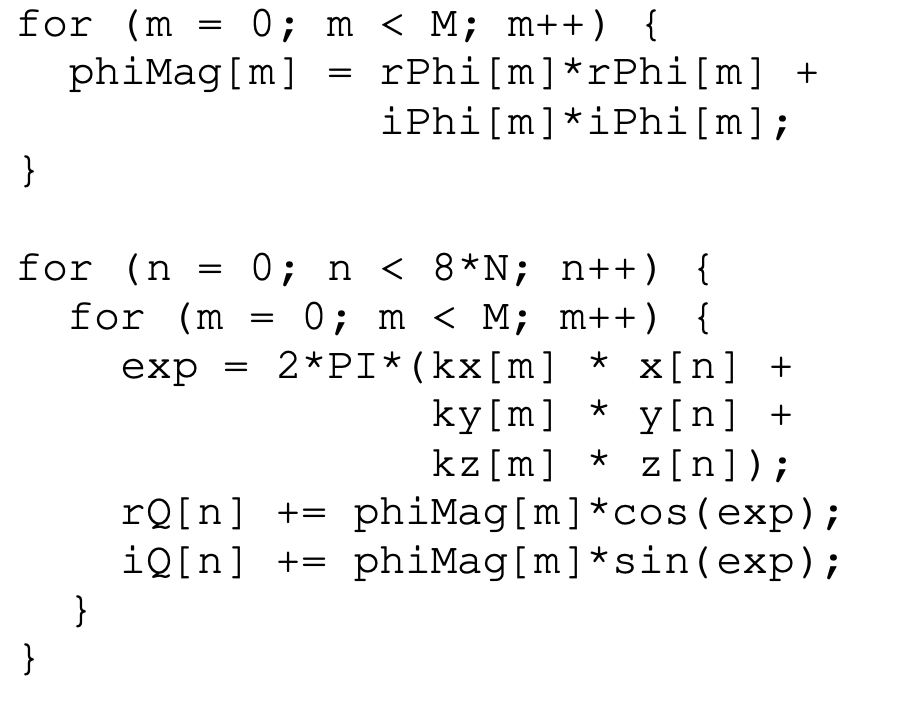
\includegraphics[width=0.85\columnwidth]{figure/algorithm-proposal.png}
\caption{Algorithm for computing MRI Q matrix~\cite{stone2008accelerating}}
\label{fig-1}
\end{figure}

\subsection{Milestones}\label{sec:arch}
\label{sec:milestones}

\vspace{-0.1in}
\begin{enumerate}
\setlength\itemsep{-0.15em}
  \item Analysis of the algorithm and the programmer's implementation in C (by Feb. 19)
  \item Learning two tutorials: "How to design an accelerator in SystemC (Cadence Stratus HLS)" and "How to design a single-core SoC"\cite{esp1}. (by Feb. 28)
  \item High-Level-Synthesis implementation in SystemC (by Mar. 11)
  \vspace{-2mm}
       \begin{itemize}
            \item Transform programmer view algorithm to HLS-ready SystemC
            \item Behavioral simulation
       \end{itemize}

  \item Baremetal application and linux application design. Evaluation on an FPGA platform (by Mar. 25)
  \item Mid-term presentation and report (by Mar. 25)
  \item Initial Design Space Exploration (by Apr. 15)
  \item Enhanced Design Space Exploration (by Apr. 22)
  \item Final refinement and analysis (by May 5)
  \item Design the same accelerator with Vivado HLS flow.
  \item Final presentation ($\sim$ May 11) and report ($\sim$ May 15)
\end{enumerate}

\subsection{Critical Aspects}
\begin{enumerate}
\setlength\itemsep{-0.15em}
\item Implement sine and cosine functions in for-loop.
\item Try different methods of optimization to reduce latency or decrease area.
\end{enumerate}



%Bibliography
{\small
\balance
%\bibliographystyle{abbrv}
\bibliographystyle{unsrt}
\bibliography{ref}
}



% If you need to add an appendix with large figures or table use the following
% code:

%% \newpage
%% \onecolumn{
%% \centering
%% \section*{APPENDIX}
%% \vspace{0.5in}

%% % Add your Appendix text and figures here.

%% }

\end{document}
